%% packages
\documentclass{article}
\usepackage[a4paper, left=2.0cm, right=2.0cm, top=3.5cm]{geometry}
\usepackage[ngerman]{babel}
\usepackage{graphicx}
\usepackage{multicol}
\usepackage{amssymb}
\usepackage{titlesec}
\usepackage{wrapfig}
\usepackage{blindtext}
\usepackage{lipsum}
\usepackage{caption}
\usepackage{listings}
\usepackage{fancyhdr}
\usepackage{nopageno}
\usepackage{authblk}
\usepackage{amsmath} % tons of math stuff
\usepackage{mathtools} % e.g. alignment within matrix
%\usepackage{bm} % provides shorthand for bold in math mode
\usepackage{dsfont} % \mathds makes double stroke digits
\usepackage{esdiff} % provides \diff
%\usepackage[ISO]{diffcoeff}
\usepackage{xcolor}
\usepackage{csquotes} % e.g. provides \enquote
\usepackage[separate-uncertainty=true]{siunitx} % units
\usepackage{xcolor} % colored text
\usepackage{csvsimple}
\usepackage{subcaption}
\usepackage{physics}
\usepackage{hyperref}
\usepackage{nameref}
\hypersetup{colorlinks=true, linkcolor=black, pdfhighlight={/N}}
\usepackage{tcolorbox}
\usepackage{amsthm}
\usepackage{float}




%\fancyhf[]{}

%% custom stuff
% own units
\DeclareSIUnit \VSS {\ensuremath{V_\mathrm{SS}}}
\DeclareSIUnit \VS {\ensuremath{V_\mathrm{S}}}
\DeclareSIUnit \Veff {\ensuremath{V_\mathrm{eff}}}
\DeclareSIUnit \Vpp {\ensuremath{V_\mathrm{pp}}}
\DeclareSIUnit \Vp {\ensuremath{V_\mathrm{p}}}
\DeclareSIUnit \VRMS {\ensuremath{V_\mathrm{RMS}}}
\DeclareSIUnit \ASS {\ensuremath{A_\mathrm{SS}}}
\DeclareSIUnit \AS {\ensuremath{A_\mathrm{S}}}
\DeclareSIUnit \Aeff {\ensuremath{A_\mathrm{eff}}}
\DeclareSIUnit \App {\ensuremath{A_\mathrm{pp}}}
\DeclareSIUnit \Ap {\ensuremath{A_\mathrm{p}}}
\DeclareSIUnit \ARMS {\ensuremath{A_\mathrm{RMS}}}

% change subsection numbering to capital letters
\newcommand{\subsectionAlph}{ \renewcommand{\thesubsection}{\arabic{section}.\Alph{subsection}} }
% change subsection numbering to lowercase letters
\newcommand{\subsectionalph}{ \renewcommand{\thesubsection}{\arabic{section}.\alph{subsection}} }
% change subsubsection numbering to lowercase letters
\newcommand{\subsubsectionalph}{ \renewcommand{\thesubsubsection}{\arabic{section}.\arabic{subsection}.\alph{subsubsection}} }
% own fig. that works with multicols
\newenvironment{Figure}
  {\par\medskip\noindent\minipage{\linewidth}}
  {\endminipage\par\medskip}
\newcommand*{\inputPath}{./plot} % prepend this command to the argument of all input commands
\graphicspath{ {./images/}{./figure/} }
% own enviroment for definitions
\newenvironment{definition}[1]
{\begin{quote} \noindent \textbf{\textit{#1\ifx&#1& \else : \fi}} \itshape}
{\end{quote}}


% own commands
% \newcommand{\rarr}{$\to\,$} %A$\,\to\,$B
\newcommand{\defc}{black}
\newcommand{\colorT}[2][blue]{\color{#1}{#2}\color{\defc}}
\newcommand{\redq}{\color{red}(?)\color{\defc}}
\newcommand{\question}[1]{\colorT[purple]{\textbf{(#1)}}}
\newcommand{\todo}[1]{\colorT[red]{\textbf{(#1)}}}
\newcommand{\mr}{\mathrm}

%% preparation
\begin{titlepage}
    \title{Praktikum Atome, Moleküle, kondensierte Materie \\ Versuch 401: Elektronische Übergänge in Atomen}
    \author[1]{Carlos Pascua\thanks{s87cpasc@uni-bonn.de}}
    \author[1]{Michael Vogt\thanks{s65mvogt@uni-bonn.de}}
    \affil[1]{Uni Bonn}
    %\date{\today}
\end{titlepage}


%% document
\begin{document}

\pagenumbering{gobble}
\maketitle
\tableofcontents
\newpage
\pagenumbering{arabic}

\pagestyle{fancy}
\fancyhead[R]{\thepage}
\fancyhead[L]{\leftmark}

\begin{multicols}{2}

\section*{Einleitung}
In diesem Versuch wird die Energieaufspaltung von Energie-Niveaus in Cadmium durch den Zeeman-Effekt untersucht.
Daraus wird das Bohrsche Magneton bestimmt sowie Eigenschaften des verwendeten Fabry-Perot-Etalons errechnet.

Anschließend wird das Franck-Hertz-Experiment durchgeführt, um die Energiedifferenz zwischen dem 6S- und 6P-Zustand von Quecksilber zu bestimmen.


\section{Zeeman-Effekt}
Im ersten Versuchsteil wird anhand einer Cadmiumlampe in einem Magnetfeld der Zeeman-Effekt auf die Zustände $^1D_2$ und $^1P_1$ untersucht.
Der verwendete Aufbau ist in Abb. \ref{fig:zeeman-aufbau} gezeigt.
\begin{figure}[H]
  \centering
  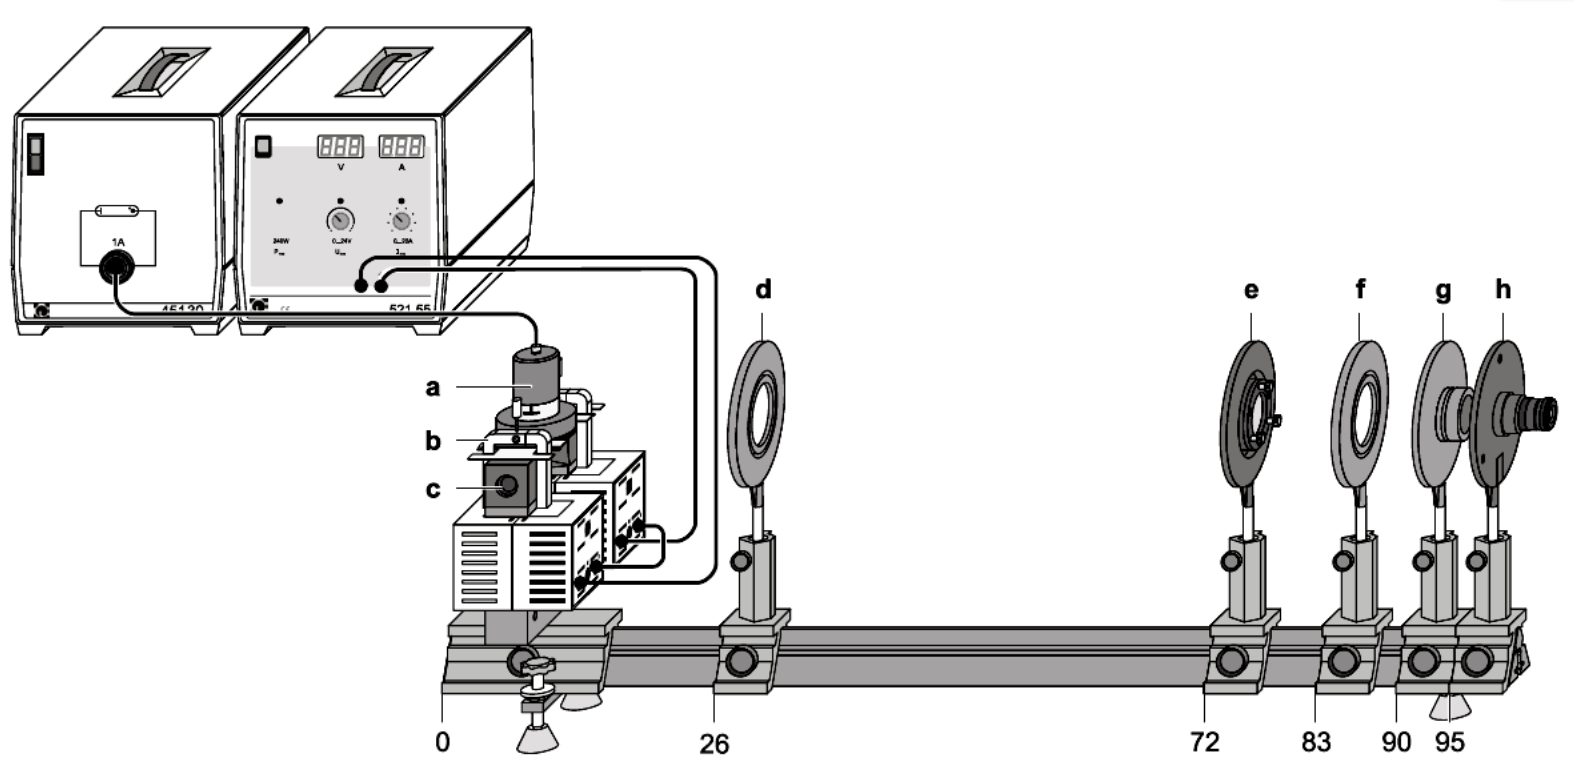
\includegraphics[width=\linewidth]{zeeman-aufbau}
  \caption{Versuchsaufbau Zeeman-Effekt \cite{Leybold}}
  \label{fig:zeeman-aufbau}
\end{figure}


\clearpage
\section{Franck-Hertz-Versuch}
Im folgenden Abschnitt wird das Franck-Hertz-Experiment durchgeführt und anschließend detailliert 
diskutiert. Anhand der durch das Cassy-Modul gemessenen Anodenstromkurven \( I_A \) wird die 
Energiedifferenz \( \Delta E \) zwischen den Energieniveaus des Quecksilbers $Hg$, \( 6S \) und \( 6P \), 
präzise bestimmt.
\subsection{Aufbau}
In einer Franck-Hertz-Röhre, die mit Quecksilbers gefüllt ist, befindet sich eine glühende 
Kathode mit einer Heisspannung $U_H$, die die Elektronen durch thermische Emmission freisetzt und in der 
Richtung einer positiv geladenen Anode beschleunigt. Die Beschleunigungsspannung $U_B$ zwischen Kathode 
und Anode bestimmt die kinetische Energie der Elektronen, bevor sie auf die Quecksilberatome treffen.

Zwischen der Kathode und der Anode befindet sich ein Gitter, das in einigen Konstruktionen mit einem kleinen 
Gegenfeld ausgestattet ist, um Elektronen, die nach elastische nd inelastische Stößen ihre kinetische Energie 
verloren haben, daran zu hindern, die Anode zu erreichen. Der Anodenstrom $I_A$
wird dann in Abhängigkeit von der Spannung $U_B$ gemessen. Bei bestimmten Spannungswerten zeigt der Anodenstrom charakteristische Einbrüche, die auftreten, wenn die Elektronen genau die Energie erreichen, die nötig ist, um ein Quecksilberatom vom Grundzustand (6S) in einen angeregten Zustand (6P) zu heben.
 Durch diesen inelastischen Stoß verlieren die Elektronen ihre kinetische Energie und tragen dadurch nicht mehr zum Stromfluss bei.

Die Spannungsdifferenz zwischen aufeinanderfolgenden Strommaxima liefert die Energie $\Delta E$, die den 
Übergang zwischen den 6S- und 6P-Niveaus beschreibt. 
\subsection{Durchführung und Auswertung}
Zunächst wird die Energiedifferenz $\Delta E$ zwischen die Energieniveaus des $Hg$ bestimmt. 
Dabei sollen die Breiten der Kurven bzw. die Peaks bestimmt werden. Dazu werden Gaußkurven an die Daten angepasst,
die mithilfe des Programms \textit{Fityk} gemacht werden.
\\ Es ist zu beachten, dass bei den verschiedenen Messungen nicht dieselbe Anzahl an Peaks 
erfasst wurde. Daher wurden nur die erkennbaren Peaks analysiert und in die Tabellen 
aufgenommen. 
\subsection*{Fityk Version 1.3.1}
In \textit{Fityk} werden Gauß-Fits durch Auswahl eines Datenbereichs und Anwendung einer Gaußfunktion als 
Modell durchgeführt. Die Gaußfunktion hat die Form 

\begin{equation*}
f(x) = a \cdot e^{-\frac{(x - \mu)^2}{2 \sigma^2}}
\end{equation*}
wobei $a$ die Amplitude, $\mu$ der Mittelwert (Zentrum des Peaks) und $\sigma$ die Standardabweichung 
ist. Das Programm optimiert die Parameter $a$, $\mu$ und $\sigma$, sodass die Abweichung zwischen dem Modell 
und den Datenpunkten minimiert wird. Die Methode der kleinsten Quadrate wird oft verwendet, um den
 Fehlerausdruck
\begin{equation*}
\sum_{i=1}^{N} (y_i - f(x_i))^2
\end{equation*}
zu minimieren, wobei $y_i$ die gemessenen Datenpunkte und $f(x_i)$ die entsprechenden Werte der Gaußfunktion 
sind. Dadurch entsteht eine Gaußkurve, die die Daten im ausgewählten Bereich bestmöglich beschreibt.
\subsection*{Diskussion der Daten}
 Wie bereits erwähnt, wurde während des Experiments nicht dieselbe Anzahl von Peaks erfasst. Dies stellt jedoch 
 kein Problem dar, da eine ausreichende Anzahl an Messwerten vorliegt. Zudem wurde in \textit{Fityk} eine 
 Hintergrundfunktion zu den Gauß-Fits hinzugefügt, sodass die Gesamtsumme der Gauß-Peaks eine bessere 
 Übereinstimmung mit den im Experiment beobachteten Peaks aufweist. Unter Berücksichtigung der oben genannten Anpassungen 
 und Messmethoden folgen nun die entsprechenden Graphen. 
\begin{figure}[H]
  \centering
  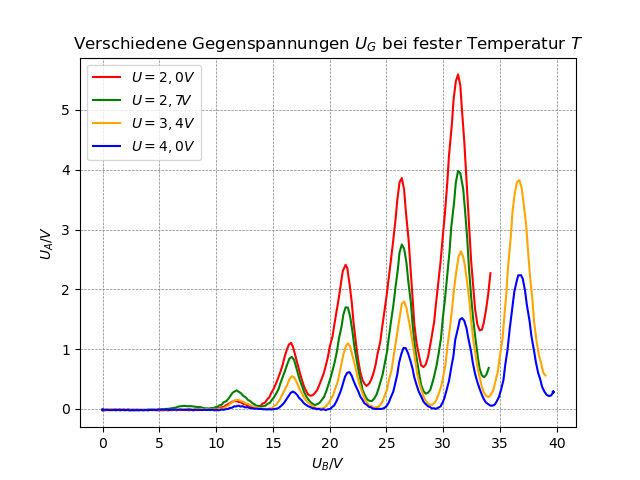
\includegraphics[scale=0.55]{FH_vieleT.png}
  \caption{Die gemessene Beschleunigungsspannung $U_B$ gegen Anodenspannung $U_A$ bei
   verschiedene Gegenspannung $T$ und fester Temperatur $U_G$}
\end{figure}
\clearpage
Nun sind auch die zugehörigen Tabellen aufgeführt.
\begin{table}[H]
  \centering
  \begin{tabular}{|c|c|c|}
      \hline
      Parameter & Wert & Fehler $\Delta$ \\ \hline
      $\mu_1$ & 31.1 & $\pm$ 0.0183 \\ \hline
      $\sigma_1$& 1.26 & $\pm$ 0.0358 \\ \hline
      $\mu_2$ & 26.1 & $\pm$ 0.0162 \\ \hline
      $\sigma_2$ & 1.08 & $\pm$ 0.0249 \\ \hline
      $\mu_3$ & 21.2 & $\pm$ 0.024 \\ \hline
      $\sigma_3$ & 0.91 & $\pm$ 0.0298 \\ \hline
      $\mu_4$ & 16.4 & $\pm$ 0.0365 \\ \hline
      $\sigma_4$ & 0.843 & $\pm$ 0.0522 \\ \hline
      $\mu_5$ & 11.7 & $\pm$ 0.237 \\ \hline
      $\sigma_5$ & 0.669 & $\pm$ 0.306 \\ \hline
  \end{tabular}
  \caption{Parameter bei $U_G=2.0V$ und $T=165^\circ C$}
  \label{tab:data_no_height}
\end{table}
\begin{table}[H]
  \centering
  \begin{tabular}{|c|c|c|}
      \hline
      Parameter & Wert & Fehler $\Delta$ \\ \hline
      $\mu_1$ & 31.3 & $\pm$ 0.00925 \\ \hline
      $\sigma_1$ & 1.04 & $\pm$ 0.0129 \\ \hline
      $\mu_2$ & 26.3 & $\pm$ 0.00979 \\ \hline
      $\sigma_2$ & 0.967 & $\pm$ 0.0151 \\ \hline
      $\mu_3$ & 21.4 & $\pm$ 0.0133 \\ \hline
      $\sigma_3$ & 0.914 & $\pm$ 0.019 \\ \hline
      $\mu_4$ & 16.6 & $\pm$ 0.0242 \\ \hline
      $\sigma_4$ & 0.885 & $\pm$ 0.0321 \\ \hline
      $\mu_5$ & 11.9 & $\pm$ 0.0715 \\ \hline
      $\sigma_5$ & 0.884 & $\pm$ 0.0916 \\ \hline
  \end{tabular}
  \caption{Parameter bei $U_G=2.7V$ und $T=165^\circ C$}
  \label{tab:data_no_height_2}
\end{table}

\begin{table}[H]
  \centering
  \begin{tabular}{|c|c|c|}
      \hline
      Parameter & Wert & Fehler $\Delta$ \\ \hline
      $\mu_1$ & 36.7 & $\pm$ 0.00818 \\ \hline
      $\sigma_1$ & 1.19 & $\pm$ 0.00971 \\ \hline
      $\mu_2$ & 31.6 & $\pm$ 0.0125 \\ \hline
      $\sigma_2$ & 1.02 & $\pm$ 0.0153 \\ \hline
      $\mu_3$ & 26.5 & $\pm$ 0.0121 \\ \hline
      $\sigma_3$ & 0.95 & $\pm$ 0.0143 \\ \hline
      $\mu_4$ & 21.6 & $\pm$ 0.0181 \\ \hline
      $\sigma_4$ & 0.871 & $\pm$ 0.0215 \\ \hline
      $\mu_5$ & 16.7 & $\pm$ 0.0362 \\ \hline
      $\sigma_5$ & 0.846 & $\pm$ 0.0423 \\ \hline
  \end{tabular}
  \caption{Parameter bei $U_G=3.4V$ und $T=165^\circ C$}
  \label{tab:data_no_height_3}
\end{table}

\begin{table}[H]
  \centering
  \begin{tabular}{|c|c|c|}
      \hline
      Parameter & Wert & Fehler $\Delta$ \\ \hline
      $\mu_1$ & 36.8 & $\pm$ 0.00835 \\ \hline
      $\sigma_1$ & 1.0 & $\pm$ 0.0123 \\ \hline
      $\mu_2$ & 31.7 & $\pm$ 0.00744 \\ \hline
      $\sigma_2$ & 0.944 & $\pm$ 0.00934 \\ \hline
      $\mu_3$ & 26.7 & $\pm$ 0.00927 \\ \hline
      $\sigma_3$ & 0.837 & $\pm$ 0.0111 \\ \hline
      $\mu_4$ & 21.7 & $\pm$ 0.0151 \\ \hline
      $\sigma_4$ & 0.769 & $\pm$ 0.0178 \\ \hline
      $\mu_5$ & 16.8 & $\pm$ 0.0313 \\ \hline
      $\sigma_5$ & 0.712 & $\pm$ 0.0371 \\ \hline
  \end{tabular}
  \caption{Parameter bei $U_G=4.0V$ und $T=165^\circ C$}
  \label{tab:data_no_height_5}
\end{table}

\begin{figure}[H]
  \centering
  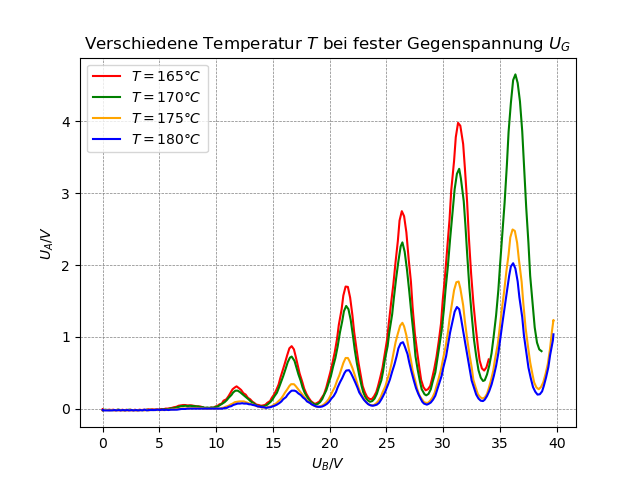
\includegraphics[scale=0.55]{FH_vieleU.png}
  \caption{Die gemessene Beschleunigungsspannung $U_B$ gegen Anodenspannung $U_A$ 
  verschiedenen Temperaturen $T$ und Gegenspannung $U_G$}
\end{figure}

\begin{table}[H]
  \centering
  \begin{tabular}{|c|c|c|}
      \hline
      Parameter & Wert & Fehler $\Delta$ \\ \hline
      $\mu_1$ & 36.3 & $\pm$ 0.00915 \\ \hline
      $\sigma_1$ & 1.11 & $\pm$ 0.0139 \\ \hline
      $\mu_2$ & 31.2 & $\pm$ 0.00858 \\ \hline
      $\sigma_2$ & 1.02 & $\pm$ 0.0136 \\ \hline
      $\mu_3$ & 26.3 & $\pm$ 0.0105 \\ \hline
      $\sigma_3$ & 0.966 & $\pm$ 0.0152 \\ \hline
      $\mu_4$ & 21.4 & $\pm$ 0.0148 \\ \hline
      $\sigma_4$ & 0.92 & $\pm$ 0.0205 \\ \hline
      $\mu_5$ & 16.6 & $\pm$ 0.0277 \\ \hline
      $\sigma_5$ & 0.889 & $\pm$ 0.0364 \\ \hline
      $\mu_6$ & 11.9 & $\pm$ 0.0832 \\ \hline
      $\sigma_6$ & 0.893 & $\pm$ 0.106 \\ \hline
  \end{tabular}
  \caption{Parameter bei $U_G=2.7V$ und $T=170^\circ C$}
  \label{tab:data_no_height_6}
\end{table}

\begin{table}[H]
  \centering
  \begin{tabular}{|c|c|c|}
      \hline
      Parameter & Wert & Fehler  \\ \hline
      $\mu_1$ & 36.3 & $\pm$ 0.128 \\ \hline
      $\sigma_1$ & 1.67 & $\pm$ 0.212 \\ \hline
      $\mu_2$ & 30.8 & $\pm$ 0.734 \\ \hline
      $\sigma_2$ & 1.08 & $\pm$ 0.26 \\ \hline
      $\mu_3$ & 26.3 & $\pm$ 0.0108 \\ \hline
      $\sigma_3$ & 0.929 & $\pm$ 0.0138 \\ \hline
      $\mu_4$ & 21.5 & $\pm$ 0.0112 \\ \hline
      $\sigma_4$ & 0.981 & $\pm$ 0.0135 \\ \hline
      $\mu_5$ & 16.8 & $\pm$ 0.0232 \\ \hline
      $\sigma_5$ & 1.00 & $\pm$ 0.0275 \\ \hline
  \end{tabular}
  \caption{Parameter bei $U_G=2.7V$ und $T=175^\circ C$}
  \label{tab:data_no_height_7}
\end{table}

\begin{table}[H]
  \centering
  \begin{tabular}{|c|c|c|}
      \hline
      Parameter & Wert & Fehler  \\ \hline
      $\mu_1$ & 36.1 & $\pm$ 0.00659 \\ \hline
      $\sigma_1$ & 0.952 & $\pm$ 0.0118 \\ \hline
      $\mu_2$ & 31.2 & $\pm$ 0.00694 \\ \hline
      $\sigma_2$ & 0.968 & $\pm$ 0.0108 \\ \hline
      $\mu_3$ & 26.3 & $\pm$ 0.0095 \\ \hline
      $\sigma_3$ & 0.921 & $\pm$ 0.0152 \\ \hline
      $\mu_4$ & 21.6 & $\pm$ 0.016 \\ \hline
      $\sigma_4$ & 0.893 & $\pm$ 0.0233 \\ \hline
      $\mu_5$ & 16.8 & $\pm$ 0.0351 \\ \hline
      $\sigma_5$ & 0.911 & $\pm$ 0.0544 \\ \hline
  \end{tabular}
  \caption{Parameter bei $U_G=2.7V$ und $T=180^\circ C$}
  \label{tab:data_no_height_8}
\end{table}
\subsection*{Bestimmung der $\Delta$Energiedifferenz}
Um die Eindeutigkeit zu gewährleisten, bezeichnen wir die Peaks bzw. die Erwartungswerte mit $U^i_B$ und 
fassen alle relevanten Informationen in einer Tabelle zusammen.
\begin{table}[H]
  \centering
  \begin{tabular}{cccccc} 
      \hline
      $U^1_B$[V] & $U^2_B$[V] & $U^3_B$[V] & $U^4_B$[V] & $U^5_B$[V] & $U^6_B$[V] \\ \hline
      36.7 & 31.1 & 26.1 & 21.2 & 16.4 & 11.7 \\ \hline
      36.8 & 31.3 & 26.3 & 21.4 & 16.6 & 11.9 \\ \hline
      36.3 & 31.6 & 26.5 & 21.6 & 16.7 & 11.9 \\ \hline
      36.3 & 31.7 & 26.7 & 21.7 & 16.6 & - \\ \hline
      36.1 & 31.2 & 26.3 & 21.4 & 16.8 & - \\ \hline
      - & 30.8 & 26.3 & 21.5 & 16.8 & - \\ \hline
      - & 31.2 & 26.3 & 21.6 & 16.8 & - \\ \hline
  \end{tabular}
  \caption{zugeordnete $U^i_B$}
  \label{tab:measurements}
\end{table}
Der Fehler des Mittelwerts wird durch die folgende Formel und in der Tabelle dargestellt:
\begin{equation*}
\Delta(U^i_B) = \sqrt{\frac{1}{N} \sum_{n=1}^{N} \left( \delta U_{i,n}^B \right)^2}
\end{equation*}
Dabei ist \( N \) die Anzahl der Werte, die zur Berechnung des Mittelwerts beitragen.
\begin{table}[H]
  \centering
  \small 
  \begin{tabular}{cccccc} 
      \hline
      $\delta U^1_B$[V] & $\delta U^2_B$[V] & $\delta U^3_B$[V] & $\delta U^4_B$[V] & $\delta U^5_B$[V] & $U^6_B$[V] \\ \hline
      $\pm 0.00818$ & $\pm 0.0183$ & $\pm 0.0162$ & $\pm 0.024$ & $\pm 0.0365$ & $\pm 0.237$ \\ \hline
      $\pm 0.00835$ & $\pm 0.00925$ & $\pm 0.00979$ & $\pm 0.0133$ & $\pm 0.0242$ & $\pm 0.0715$ \\ \hline
      $\pm 0.00915$ & $\pm 0.0125$ & $\pm 0.0121$ & $\pm 0.0181$ & $\pm 0.0362$ & $\pm 0.0832$ \\ \hline
      $\pm 0.128$ & $\pm 0.00744$ & $\pm 0.00927$ & $\pm 0.0151$ & $\pm 0.0313$ & - \\ \hline
      $\pm 0.00659$ & $\pm 0.00858$ & $\pm 0.0105$ & $\pm 0.0148$ & $\pm 0.0277$ & - \\ \hline
      - & $\pm 0.734$ & $\pm 0.0108$ & $\pm 0.0112 $ & $\pm 0.0232$ & - \\ \hline
      - & $\pm 0.00694$ & $\pm 0.0095$ & $\pm 0.016$ & $\pm 0.0351$ & - \\ \hline
  \end{tabular}
  \caption{zugeordnete $\delta U^i_B$}
  \label{tab:measurements}
\end{table}
Im Folgenden sind die Mittelwerte der Beschleunigungsspannung sowie die entsprechenden Fehler dargestellt.
\begin{table}[H]
  \centering
  \begin{tabular}{cc} 
      \hline
      & Mittelwert [V] \\ \hline
      $U^1_B$ & 36.3 \\ \hline
      $U^2_B$ & 31.2 \\ \hline
      $U^3_B$ & 26.3 \\ \hline
      $U^4_B$ & 21.6 \\ \hline
      $U^5_B$ & 16.6 \\ \hline
      $U^6_B$ & 11.8 \\ \hline
  \end{tabular}
  \caption{Mittelwerte zu $U^i_B$}
  \label{tab:median_values}
\end{table}

\begin{table}[H]
  \centering
  \begin{tabular}{cc} 
      \hline
       & Mittelwert [V] \\ \hline
      $\delta U^1_B$ & $\pm 0.0504$ \\ \hline
      $\delta U^2_B$ & $\pm 0.133$ \\ \hline
      $\delta U^3_B$ & $\pm 0.0112$ \\ \hline
      $\delta U^4_B$ & $\pm 0.0161$ \\ \hline
      $\delta U^5_B$ & $\pm 0.0307$ \\ \hline
      $\delta U^6_B$ & $\pm 0.131$ \\ \hline
  \end{tabular}
  \caption{Mittelwerte zu $\delta U^i_B$}
  \label{tab:mean_values}
\end{table}
Nun kann man aus den Diferenzen der benachbaren Peaks der Energiedifferenz $\Delta E$ bestimmt werden. 
\begin{equation*}
  \Delta E=(4.9 \pm 0.0803)eV
\end{equation*}
Das Ergebnis unserer experimentellen Messungen ist äußerst erfreulich und stimmt vollständig 
mit dem erwarteten theoretischen Wert der Übergang zwischen $6^1 S_o \rightarrow 6^3P_1$ überein. 
Wie man in der Abbildung sich anschauen kann. 
\clearpage
\begin{figure}[H]
  \centering
  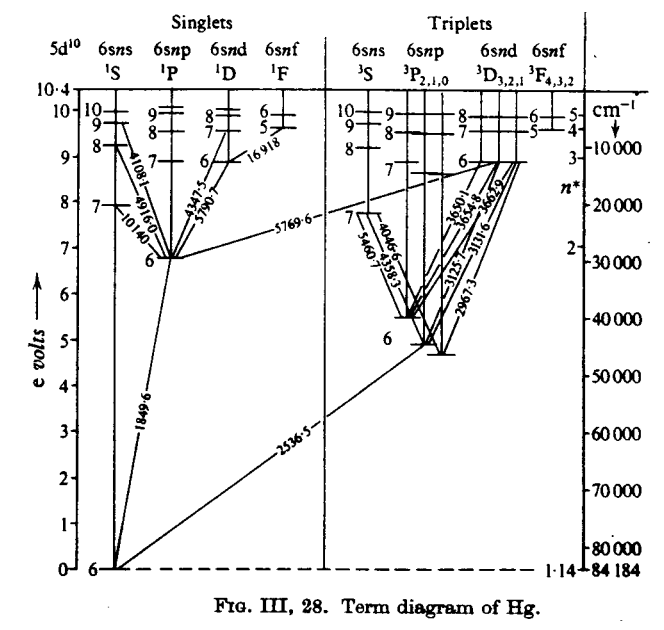
\includegraphics[scale=0.45]{Vereinfachtes Hg-Termschema.png}
  \caption{Termschema des Quecksilbers}
\end{figure}
\subsection{Einfluss der Temperatur $T$ und der Gegenspannung $U_2$}
\begin{figure}[H]
  \centering
  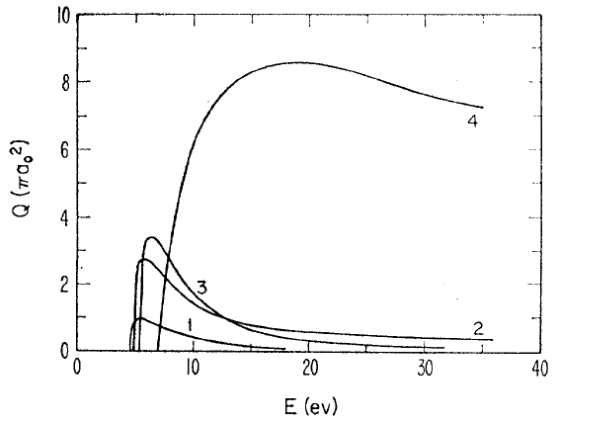
\includegraphics[scale=0.55]{Totaler Wirkungsquerschnitt.png}
  \caption{Totaler Wirkungsquerschnitt $Q(\pi a^2_0$) von Hg für Elektronenstoßanregung}
\end{figure}
\section{Fazit}
\clearpage
\begin{thebibliography}{9}

\bibitem{Anleitung}
\textit{Physikalisches Praktikum Teil IV -- Versuchsbeschreibungen}, Universität Bonn, Abruf 29.10.2024

\bibitem{Leybold}
\textit{Beobachtung des normalen Zeeman-Effekts in transversaler und longitudinaler Konfiguration}, Leybold Didactic, Abruf 30.10.2024

\end{thebibliography}

\end{multicols}

\end{document}

